\chapter*{Visualization}
In this section we provide an analysis of the data in terms of their
graphical representation and visualization.\\

\section*{Histograms}
We ploted a histogram for each attribute to investigate its distribution. 
Each histogram shows how many records had a value of attribute in a range
of particular bucket.

\begin{figure}[!tbh]
	\centering
	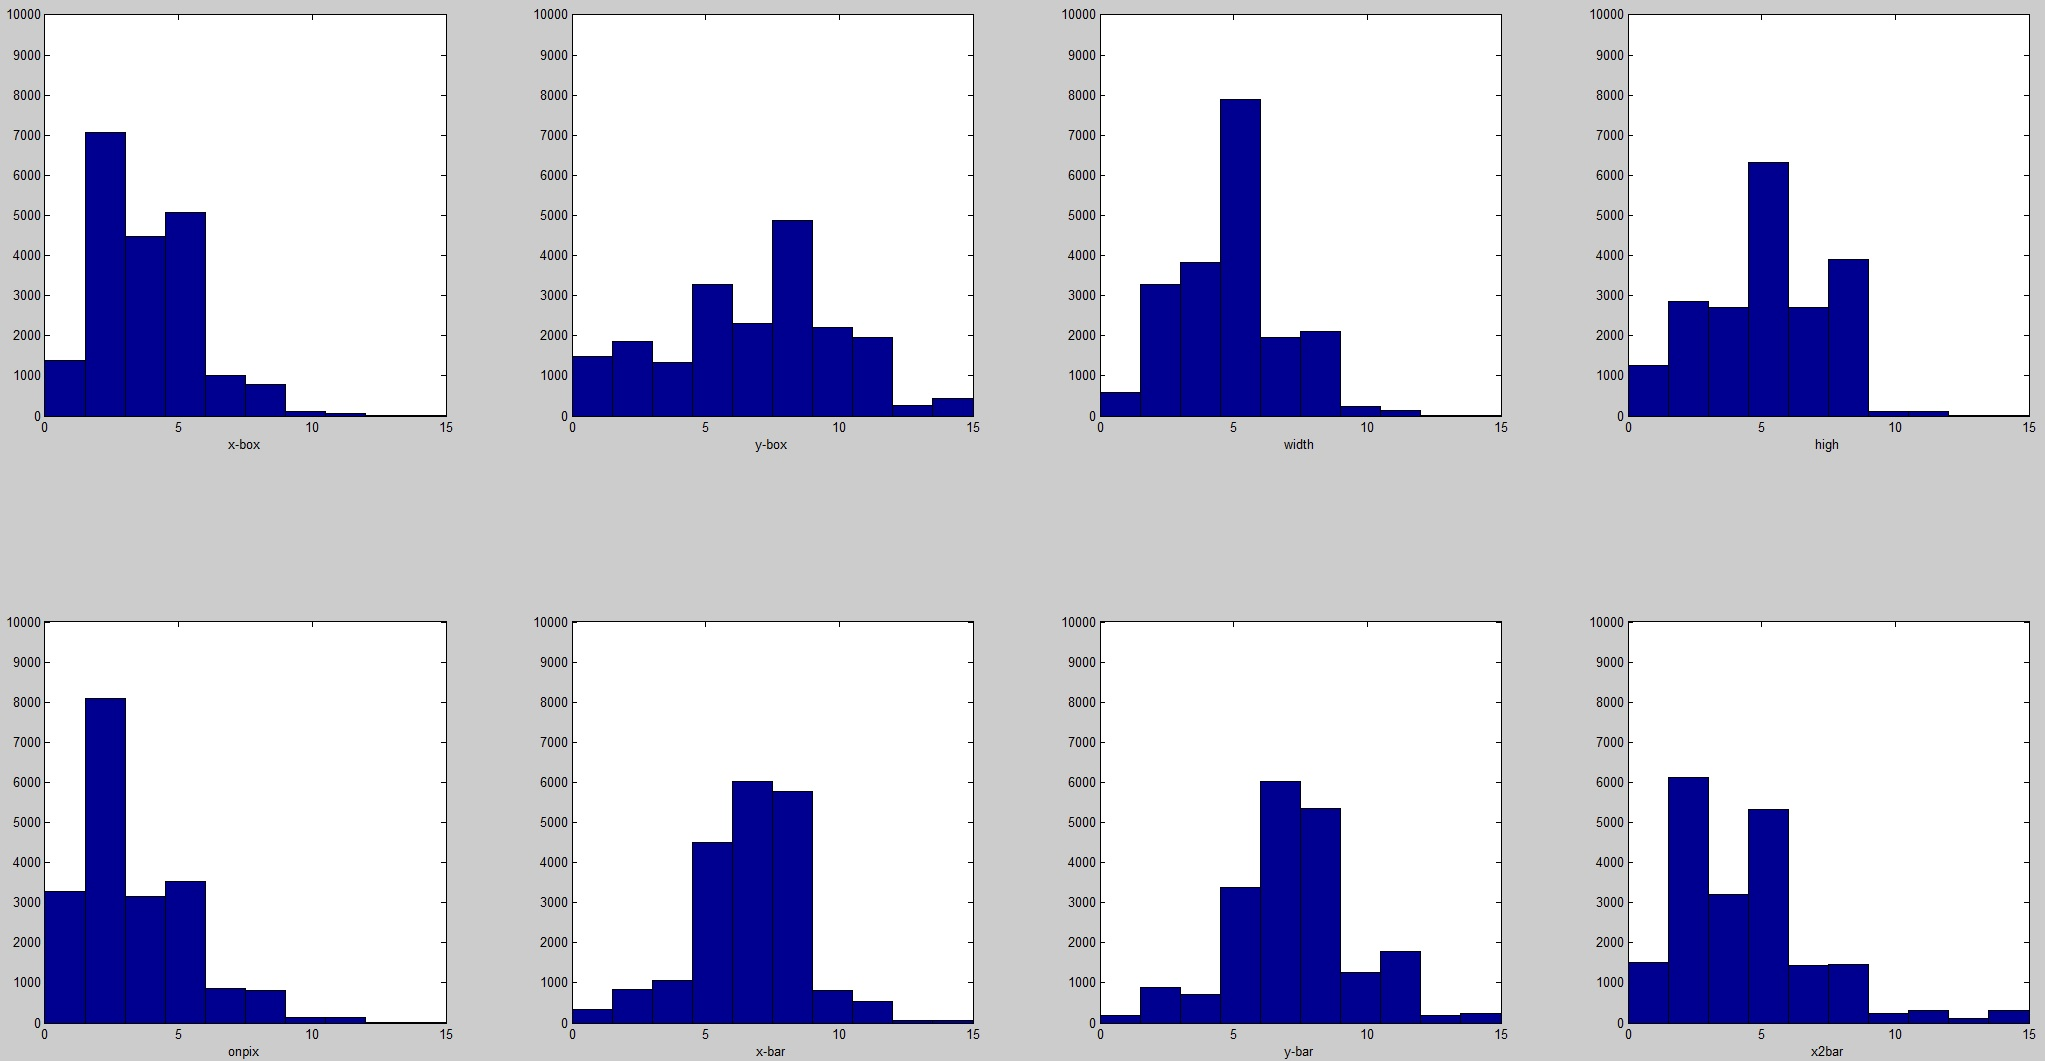
\includegraphics[width=1\textwidth]{figures/histograms_1}
	\caption{Histograms for first attributes 0-7}
	\label{fig:histograms_1}
\end{figure}

\begin{figure}[!tbh]
	\centering
	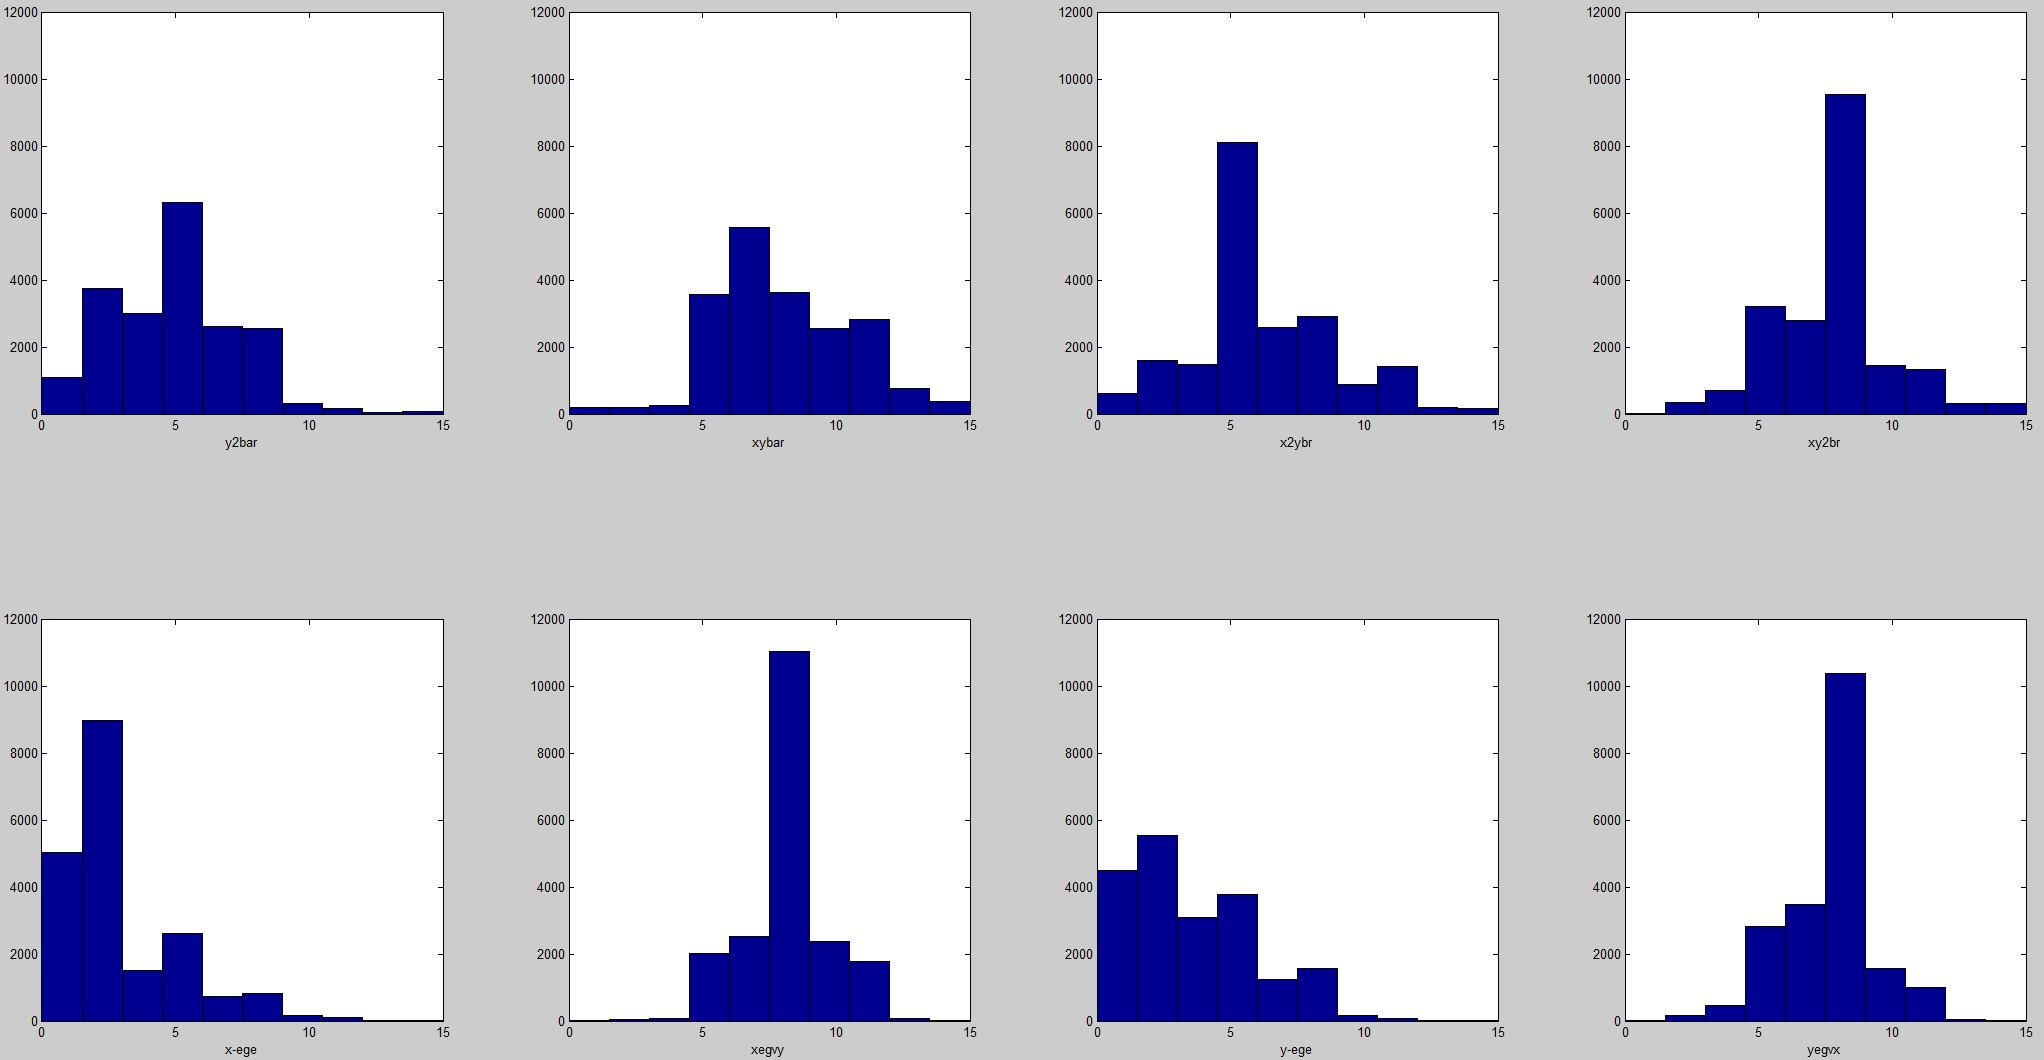
\includegraphics[width=1\textwidth]{figures/histograms_2}
	\caption{Histograms for first attributes 8-15}
	\label{fig:histograms_2}
\end{figure}

\section*{Box plots}

\begin{figure}[!tbh]
	\centering
	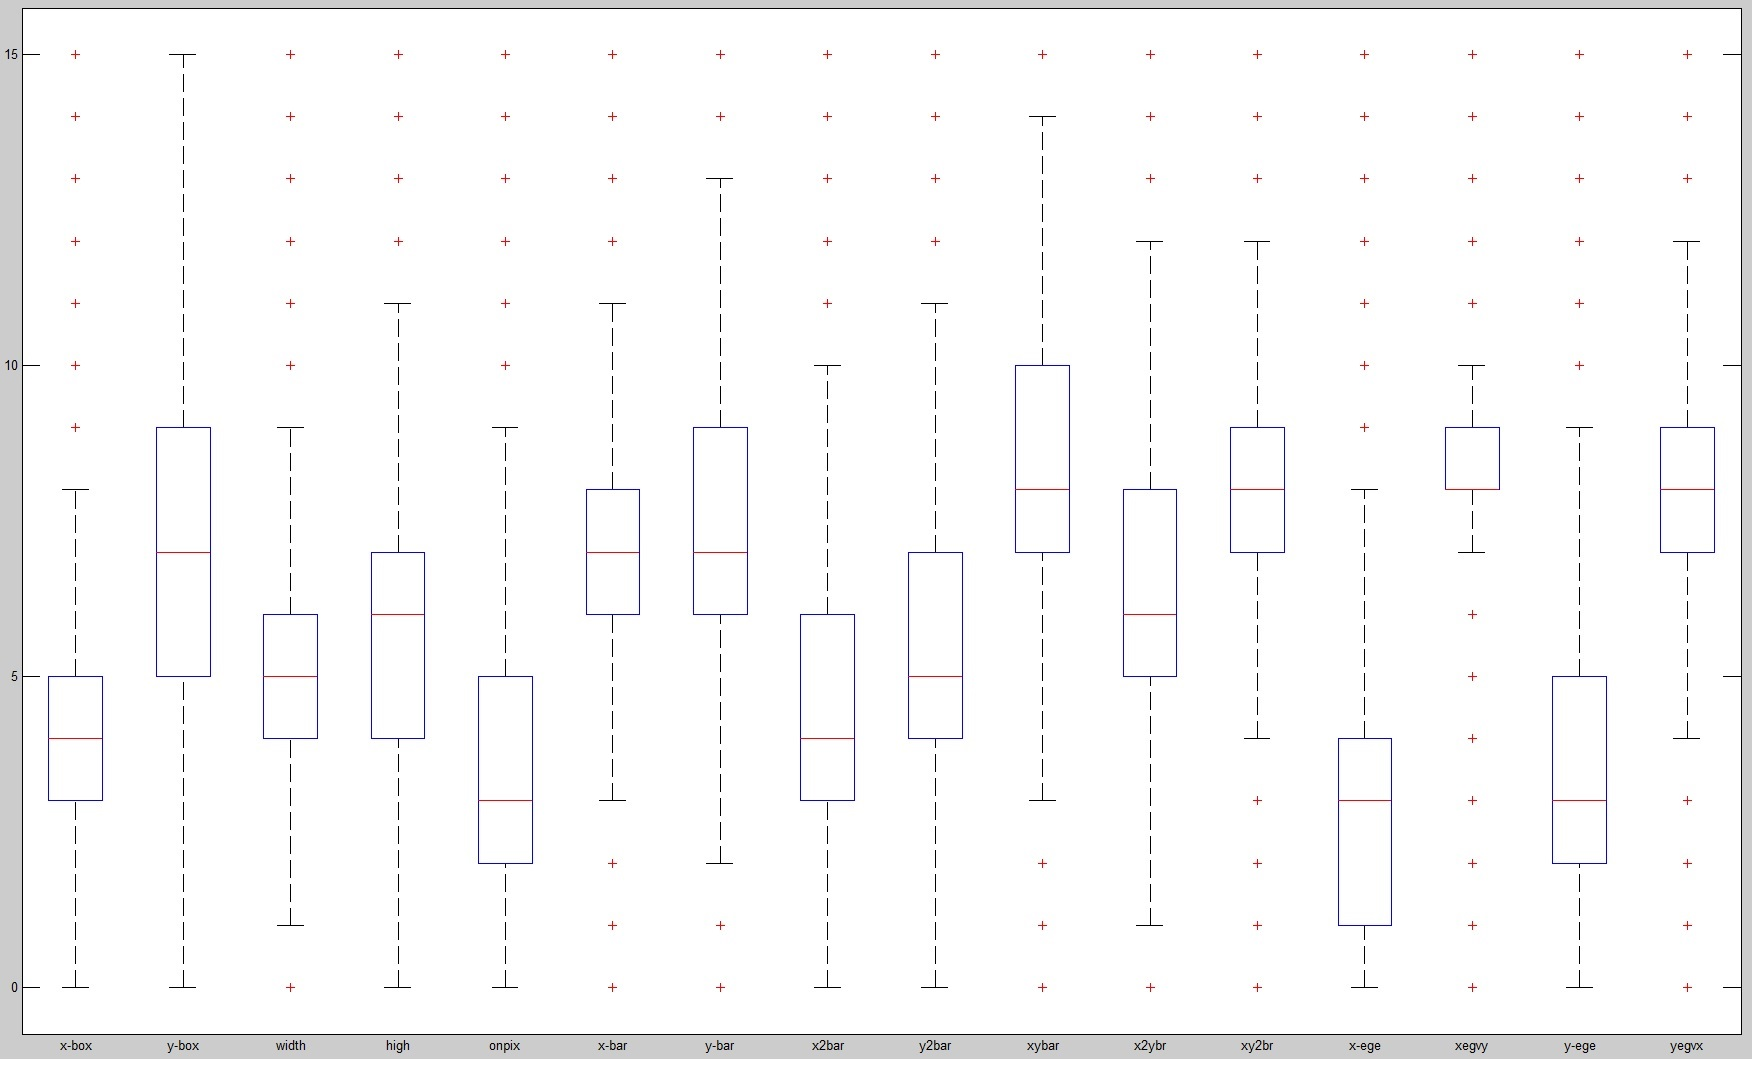
\includegraphics[width=1\textwidth]{figures/boxplot_all}
	\caption{Box plot for all records of the data set}
	\label{fig:boxplot_all}
\end{figure}

\begin{figure}[!tbh]
	\centering
	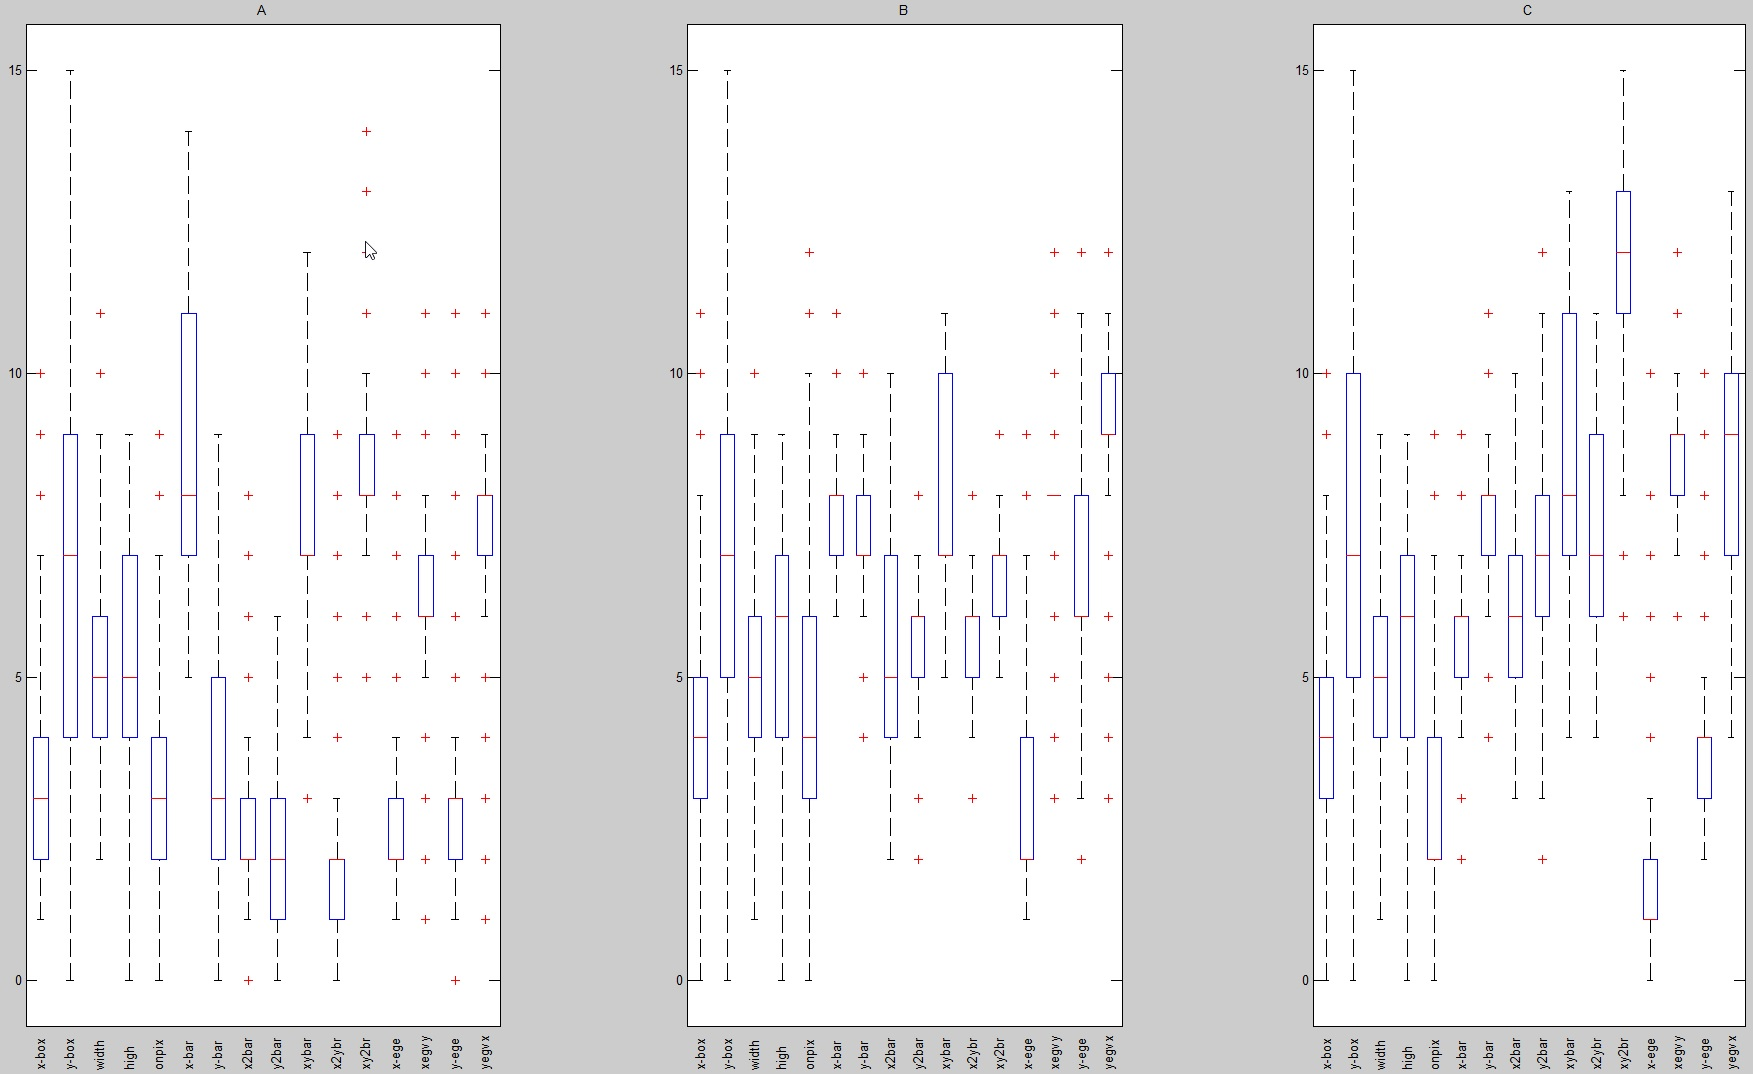
\includegraphics[width=1\textwidth]{figures/boxplot_perclass}
	\caption{Box plot for classes A,B,C of the data set}
	\label{fig:boxplot_perclass}
\end{figure}

\section*{PCA}

\subsection*{Variance}

\begin{figure}[!tbh]
	\centering
	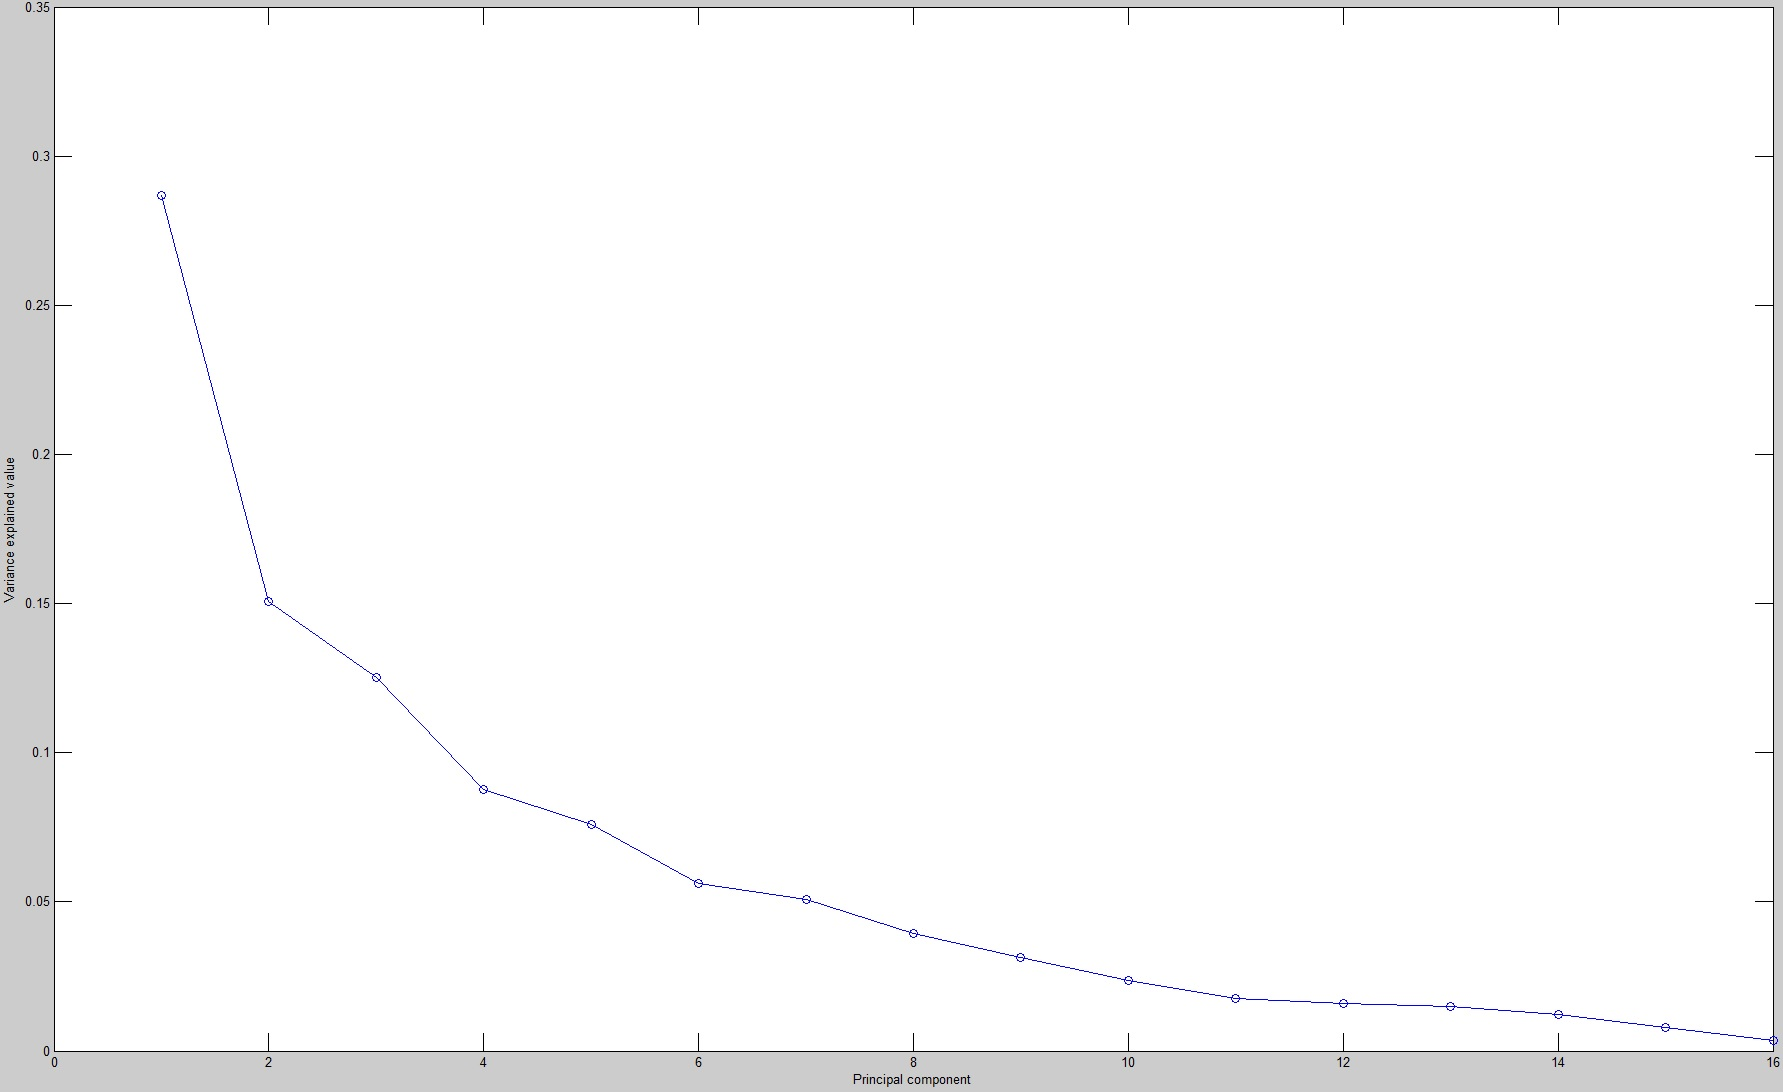
\includegraphics[width=1\textwidth]{figures/variance_perpc}
	\caption{Variance represented by each principal component}
	\label{fig:variance_perpc}
\end{figure}

\begin{figure}[!tbh]
	\centering
	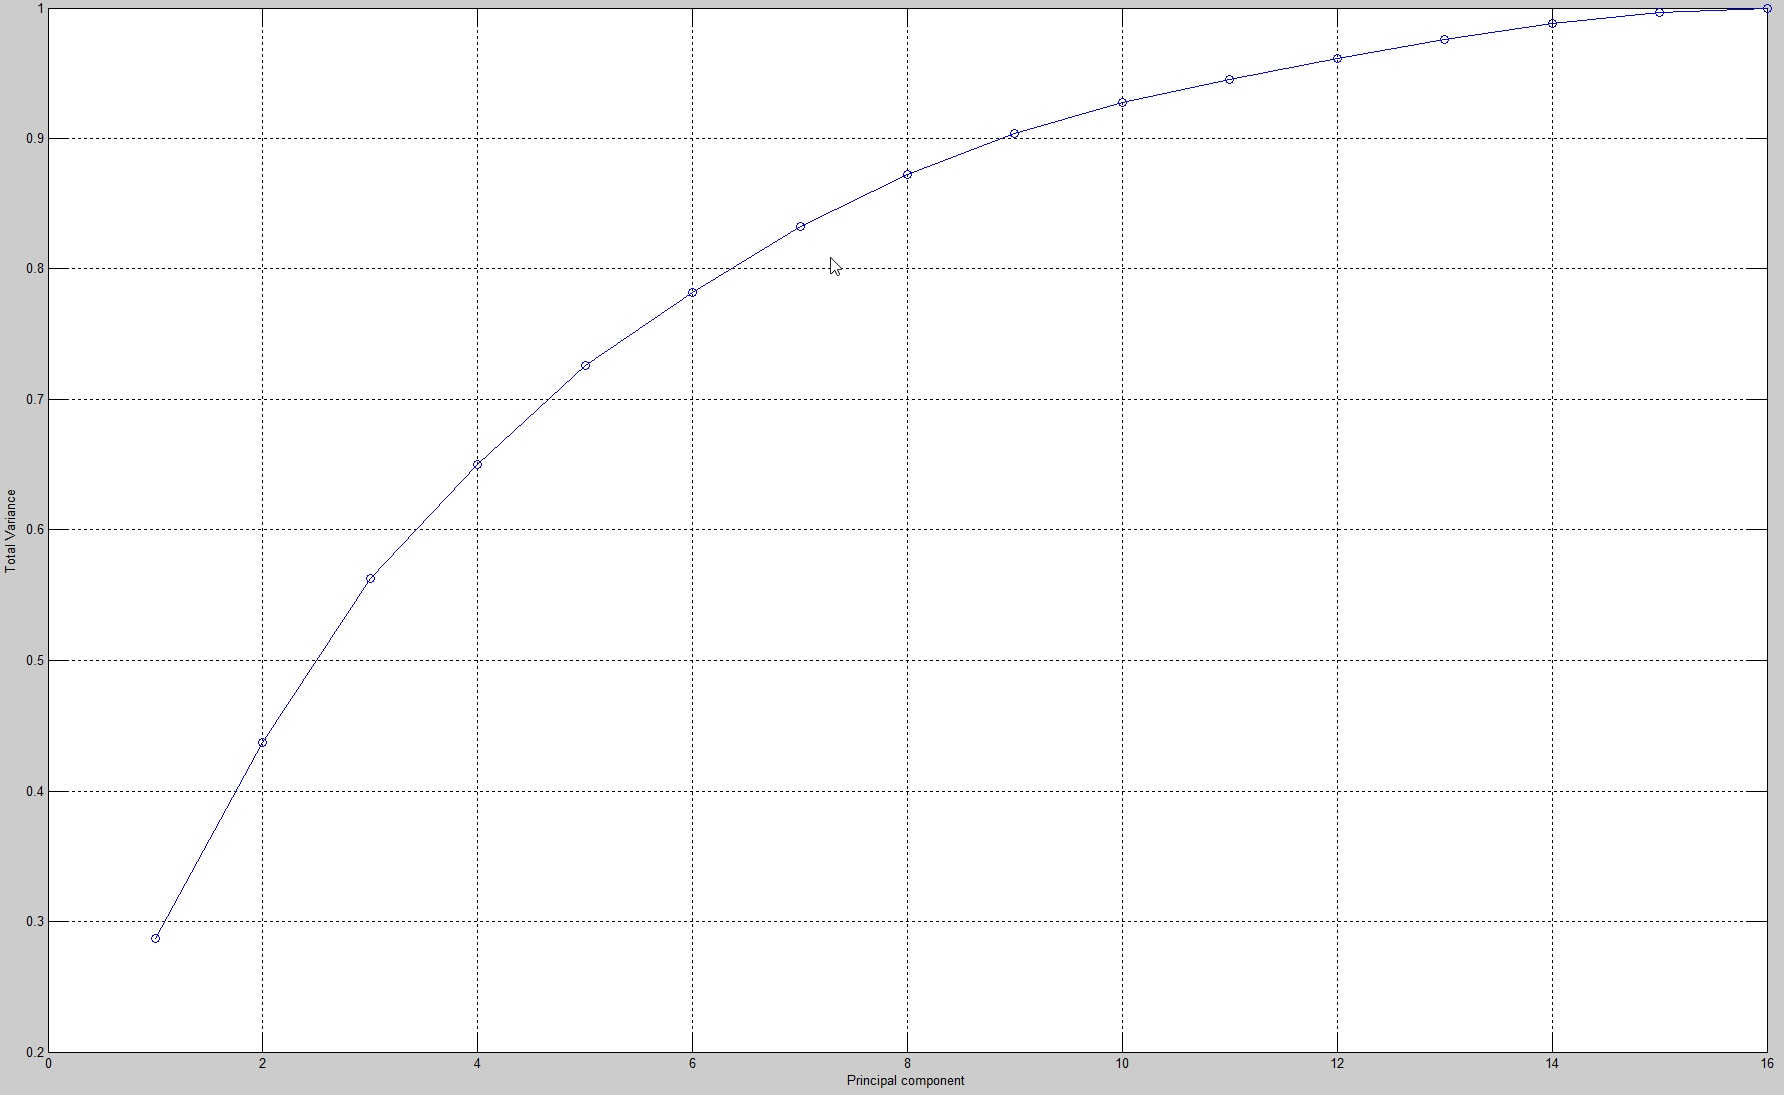
\includegraphics[width=1\textwidth]{figures/variance_cummulated}
	\caption{Cummulative variance for principal components}
	\label{fig:boxplot_cummulated}
\end{figure}

\subsection*{PCA - visualization}

\begin{figure}[!tbh]
	\centering
	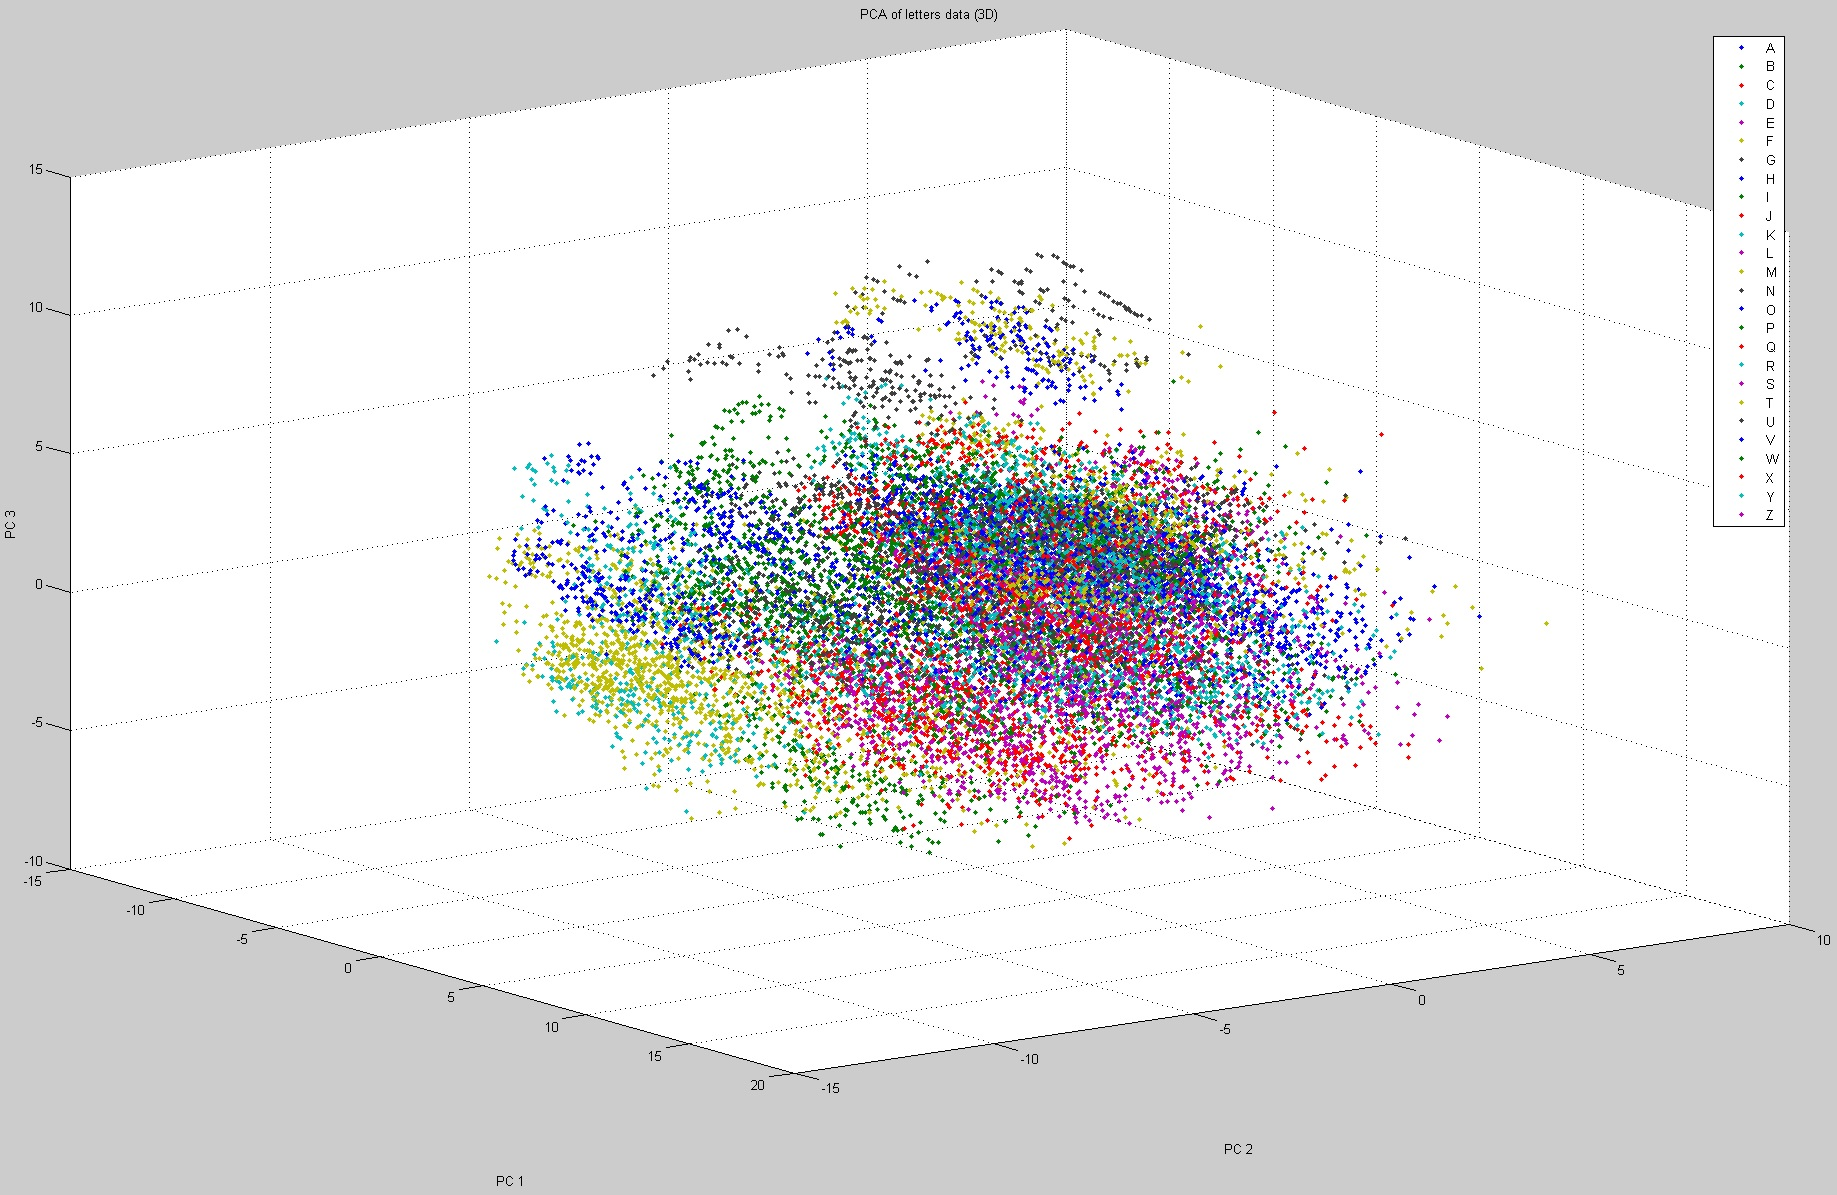
\includegraphics[width=1\textwidth]{figures/pca_points_all_3D}
	\caption{All the data set represented by first 3 PC}
	\label{fig:pca_points_all_3D}
\end{figure}

\begin{figure}[!tbh]
	\centering
	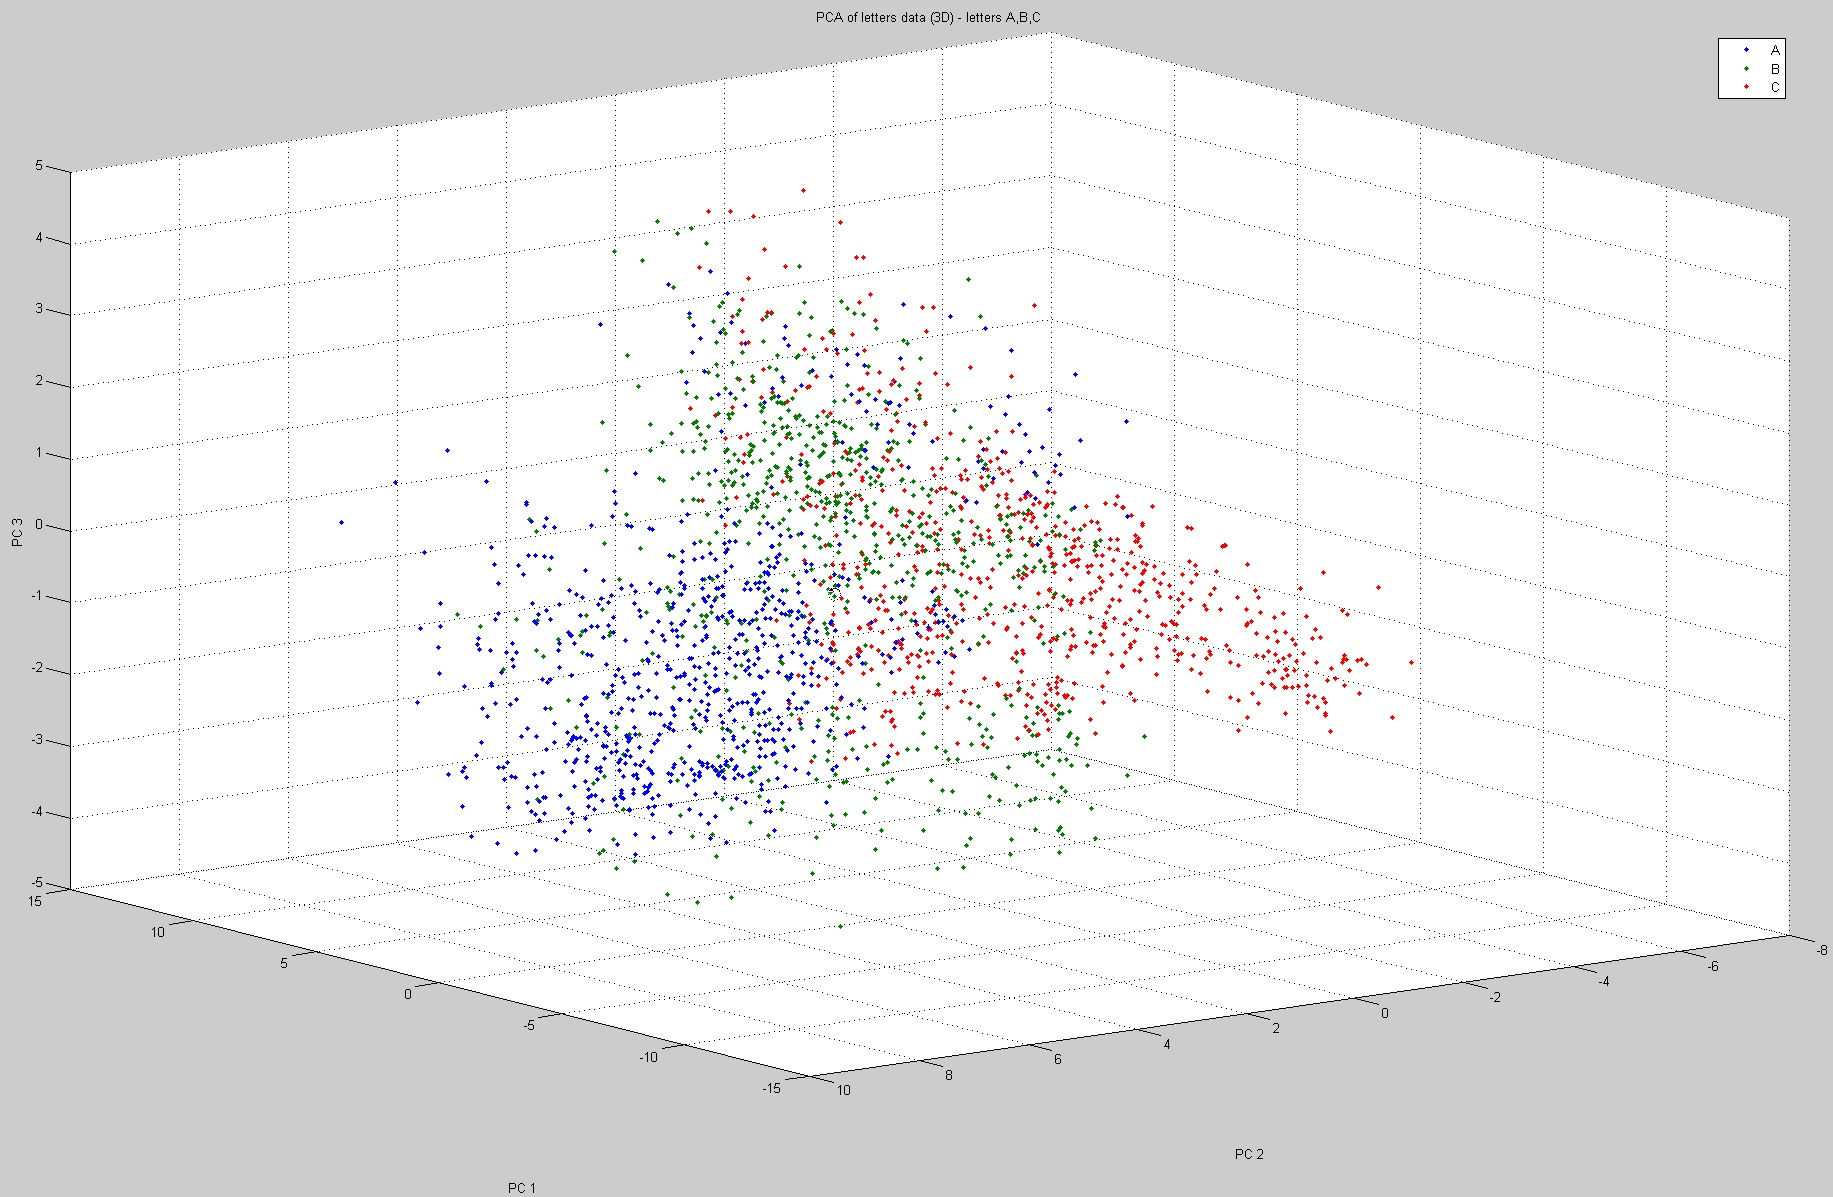
\includegraphics[width=1\textwidth]{figures/pca_points_abc_3D}
	\caption{Classes A,B and C represented by first 3 PC}
	\label{fig:pca_points_abc_3D}
\end{figure}